\documentclass[12pt,a4paper]{article}

\newcommand{\TETELNUMBER}{9}
\newcommand{\TETELTITLE}{Topológiák, kommunikációs modellek és aszinkron programozás}
\newcommand{\TETELSHORTTITLE}{Topológiák és async modellek}

\newcommand{\ZVTetelsorDataOnly}{}
\newcommand{\ZVTetelOne}{Adatok, adattípusok, adatműveletek és adatstruktúrák. Szám adattípus. Számrendszerek, konverziók. A logikai, halmaz, karakter, sztring absztrakt adattípusok és realizációjuk. A tömb (vektor, mátrix), rekord absztrakt adattípusok.}
\newcommand{\ZVTetelTwo}{Az algoritmus. Iteratív és rekurzív algoritmus. A számítógépes memória. Adat és program. Verem és procedúra. Az algoritmus lejegyzése. A folyamatábra és a pszeudokód. Elemi algoritmusok.}
\newcommand{\ZVTetelThree}{Strukturált programozás. Programgráf, valódi program, vezérlőgráf lebontása, strukturált program és annak formulája. Strukturált programgráf kialakítása, struktogram. Ciklikus bonyolultság és egyéb bonyolultsági tételek.}
\newcommand{\ZVTetelFour}{Számelméleti algoritmusok. Legnagyobb közös osztó, euklideszi és kibővített euklideszi algoritmus, lineáris kongruencia egyenletek. Multiplikatív inverz, moduláris hatványozás, Fermat prímteszt. RSA.}
\newcommand{\ZVTetelFive}{Rendezések: Beszúró rendezés. Az ,,Oszd meg és uralkodj!'' elv. Összefésülő rendezés. Gyors rendezés. Buborék rendezés. Shell rendezés. Minimum kiválasztásos rendezés. Négyzetes rendezés. Lineáris idejű rendezések: leszámláló rendezés, számjegyes rendezés. Időelemzéseik. Az összehasonlító rendezések időtétele.}
\newcommand{\ZVTetelSix}{Gráfalgoritmusok. Szélességi keresés. Mélységi keresés. Topologikus rendezés. Optimumfeladatok fákon (minimális feszítőfák, Kruskal- és Prim-algoritmus). Legrövidebb utak meghatározása (Dijkstra-algoritmus, Bellman--Ford-algoritmus, Floyd--Warshall-algoritmus).}
\newcommand{\ZVTetelSeven}{A párhuzamos algoritmusok alapfogalmai, PRAM modell, hatékonysági mértékek (munka, költség, gyorsítás, hatékonyság). Párhuzamos végrehajtás ábrázolási módjai. Komplexitás becslése, párhuzamos komplexitás. Amdahl törvénye. Pipeline párhuzamosítás, Lost update probléma bemutatása és megoldása.}
\newcommand{\ZVTetelEight}{Aggregáció, redukció, prefixszámítás párhuzamosítási lehetőségei. \texttt{CREW\_PREFIX}, \texttt{EREW\_PREFIX} és \texttt{OPTIMAL\_PREFIX} algoritmusok bemutatása. Összefésülő rendezés párhuzamosítási módja.}
\newcommand{\ZVTetelNine}{A busz, gyűrű, rács, tórusz, hiperkocka és fa topológiák bemutatása, csomópontok közötti távolságok jellemzése. A CSP, Publish--Subscribe és az Aktor modell. Az aszinkron programozás elemei: async, await kulcsszavak használata, coroutine-ok.}
\newcommand{\ZVTetelTen}{A Turing-gép fogalma, működése. A RAM-gép. Boole-függvények és logikai hálózatok.}
\newcommand{\ZVTetelEleven}{Algoritmikus eldönthetőség. Church-tézis. Rekurzív és rekurzívan felsorolható nyelvek, rekurzív illetve parciálisan rekurzív függvények. Nevezetes nyelvek (Az R, Re, coR, coRE nyelvosztályok és ezek kapcsolata) és bonyolultságuk. Algoritmikusan eldönthetetlen problémák. Polinomiális idejű algoritmusok.}
\newcommand{\ZVTetelTwelve}{Nemdeterminisztikus Turing-gépek, az NP és a coNP nyelvosztály. Példák NP-beli nyelvekre. A tanú-tétel. Nemdeterminisztikus algoritmusok bonyolultsága. NP-teljesség, Cook-tétel. Néhány NP-teljes probléma, Cook--Levin-tétel.}
\newcommand{\ZVTetelThirteen}{A Java programozási nyelv története, alapvető jellemzői. Egy Java program szerkezete (csomagok és fordítási egységek). Az objektumorientált programtervezés alapelveinek felsorolása. Objektumok tárolása és élettartama. Szemétgyűjtő mechanizmus. Kivételkezelés.}
\newcommand{\ZVTetelFourteen}{Az egységbezárás és az információrejtés objektumorientált alapelvek megvalósítása. Osztálydefiníció és példányosítás. Osztályszintű és példányszintű tagok, konstansok. Hozzáférési kategóriák és használatuk. Hivatkozás az osztály tagjaira.}
\newcommand{\ZVTetelFifteen}{Az öröklődés és a polimorfizmus objektumorientált alapelvek megvalósítása. Öröklődés szabályai, metódusok túlterhelése és felüldefiniálása. A referencia statikus és dinamikus típusa. Absztrakt osztály és interfész szerepe, összehasonlítása.}
\newcommand{\ZVTetelSixteen}{Az operációs rendszerbeli folyamat (processz) fogalma. Folyamatkontextus. A fonál (szál) fogalma. A processzállapotok, állapotváltások, processz futási módok. Taszk- és fonálállapotok, állapotátmenetek.}
\newcommand{\ZVTetelSeventeen}{A memóriamenedzselés feladatai. Memória mint erőforrás. Címleképzés fajtái. Lapozós virtuális memóriamenedzselés működése. Allokálás, nyilvántartás, címleképzés. Laphiba fogalma, kezelése, kilapozási stratégiák. Előnyök, hátrányok.}
\newcommand{\ZVTetelEighteen}{Fájlrendszer-megvalósítási feladatok. Jegyzékszerkezetek. Szabadblokk-menedzselési lehetőségek. Fájlattribútum-rögzítési lehetőségek (ezen belül a fájltestet képező blokkok rögzítési lehetőségei).}
\newcommand{\ZVTetelNineteen}{Relációs adatmodell, relációs struktúra és integritási feltételek. ER modell elemei jelentése és jelölése. Az ER modell konverziója relációs modellre. Relációs adatmodell műveleti része, relációs algebra.}
\newcommand{\ZVTetelTwenty}{Az SQL szabvány relációs adatbázis kezelő nyelv bemutatása, a DDL (objektum létrehozás, megszüntetés és szerkezet módosítás), DML (rekord felvitel, törlés és módosítás), DCL és a SELECT utasítások áttekintése és használata. Beágyazott SELECT használata. A relációs algebra műveleteinek megvalósítása SQL-ben.}
\newcommand{\ZVTetelTwentyOne}{Adatkezelés és adatbáziskezelés alapfogalmai, fileszervezési módszerek, B-fa index; adatbázis architektúra; A normalizálás szerepe a relációs adatbázis kezelésben. Redundancia oka és a megszüntetés lépései. Normálformák. Dekompozíció célja és szabályai, tételei.}
\newcommand{\ZVTetelTwentyTwo}{Számítógép-hálózatokhoz kötődő alapfogalmak és az ISO--OSI hivatkozási modell: topológia és méret szerinti osztályozásuk. Kapcsolástechnika szerinti osztályozásuk (vonalkapcsolás, üzenetkapcsolás, csomagkapcsolás és virtuális vonalkapcsolás). Az ISO--OSI hivatkozási modell szerkezete, rétegei és azok főbb funkciói.}
\newcommand{\ZVTetelTwentyThree}{A számítógép-hálózatok ISO--OSI hivatkozási modell adatkapcsolati rétegének közeghozzáférési alrétege: A főbb csatorna-megosztási osztályok (statikus-dinamikus, dinamikus versengő-determinisztikus) bemutatása és azok összevetése. Az IEEE 802.3 és az Ethernet (CSMA/CD) keretformátum, MAC címek, támogatott közegek és sebességek bemutatása, működés duplex csatorna esetén. Az IEEE 802.11 WLAN általános felépítése, az Access Point (AP) főbb funkciói. Az alkalmazott közeghozzáférési módszer (CSMA/CA), Distributed Coordination Function (DCF) és Point Coordination Function (PCF) üzemmódok.}
\newcommand{\ZVTetelTwentyFour}{A TCP/IP protokollszövet és az Internet. Az Internet hivatkozási modell (DoD) és az ISO--OSI hivatkozási modell összevetése. A TCP/IP protokollszövet főbb részei (ARP, RARP, IP, ICMP, TCP, UDP) és azok funkciói. Az internetes címzés és címosztályok: IPv4-címosztályok, maszk, subnet, supernet, osztály nélküli címzés (CIDR -- Classless Inter-Domain Routing) és változó alhálózat-méretek (VLSM -- Variable Length Subnet Mask), címek kiosztása, lokális címek és címfordítás (NAT). IPv6-címek, IPv6-címtípusok (unicast, multicast, anycast; link local, unique local, aggregatable global unicast address).}
\newcommand{\ZVTetelTwentyFive}{Szoftvertechnológia és a szoftverfolyamat fogalma. A szoftverfolyamat-fázisok részletes bemutatása: szoftverspecifikáció, tervezés, implementáció, validáció és evolúció. Az evolúciós modell ismertetése.}
\newcommand{\ZVTetelTwentySix}{Szoftverkövetelmény fogalma és osztályozásai. Követelmények általános problémái. Követelményfeltárás és -elemzés folyamata. Vezérlési stílusok.}
\newcommand{\ZVTetelTwentySeven}{UML diagramok bemutatása: Use case és osztálydiagram. A szekvenciadiagram. Komponensdiagram.}

\newcommand{\ZVTetelKiiras}[1]{%
  \ifcase#1\relax
  \or \ZVTetelOne
  \or \ZVTetelTwo
  \or \ZVTetelThree
  \or \ZVTetelFour
  \or \ZVTetelFive
  \or \ZVTetelSix
  \or \ZVTetelSeven
  \or \ZVTetelEight
  \or \ZVTetelNine
  \or \ZVTetelTen
  \or \ZVTetelEleven
  \or \ZVTetelTwelve
  \or \ZVTetelThirteen
  \or \ZVTetelFourteen
  \or \ZVTetelFifteen
  \or \ZVTetelSixteen
  \or \ZVTetelSeventeen
  \or \ZVTetelEighteen
  \or \ZVTetelNineteen
  \or \ZVTetelTwenty
  \or \ZVTetelTwentyOne
  \or \ZVTetelTwentyTwo
  \or \ZVTetelTwentyThree
  \or \ZVTetelTwentyFour
  \or \ZVTetelTwentyFive
  \or \ZVTetelTwentySix
  \or \ZVTetelTwentySeven
  \fi
}

\newcommand{\ZVTetelsorList}{%
\begin{enumerate}[leftmargin=7mm,label=\arabic*.,itemsep=2pt,topsep=2pt,parsep=0pt]
  \item \ZVTetelOne
  \item \ZVTetelTwo
  \item \ZVTetelThree
  \item \ZVTetelFour
  \item \ZVTetelFive
  \item \ZVTetelSix
  \item \ZVTetelSeven
  \item \ZVTetelEight
  \item \ZVTetelNine
  \item \ZVTetelTen
  \item \ZVTetelEleven
  \item \ZVTetelTwelve
  \item \ZVTetelThirteen
  \item \ZVTetelFourteen
  \item \ZVTetelFifteen
  \item \ZVTetelSixteen
  \item \ZVTetelSeventeen
  \item \ZVTetelEighteen
  \item \ZVTetelNineteen
  \item \ZVTetelTwenty
  \item \ZVTetelTwentyOne
  \item \ZVTetelTwentyTwo
  \item \ZVTetelTwentyThree
  \item \ZVTetelTwentyFour
  \item \ZVTetelTwentyFive
  \item \ZVTetelTwentySix
  \item \ZVTetelTwentySeven
\end{enumerate}%
}


\newcommand{\tetelsorrow}[2]{\textbf{#1.} & #2\tabularnewline}

\newcommand{\tetelsorpageone}{%
\begin{tabularx}{\textwidth}{|>{\raggedleft\bfseries}p{8mm}@{\hspace{5mm}}>{\raggedright\arraybackslash}X|}
\hline
\tetelsorrow{1}{\ZVTetelOne}
\tetelsorrow{2}{\ZVTetelTwo}
\tetelsorrow{3}{\ZVTetelThree}
\hline
\tetelsorrow{4}{\ZVTetelFour}
\tetelsorrow{5}{\ZVTetelFive}
\tetelsorrow{6}{\ZVTetelSix}
\hline
\tetelsorrow{7}{\ZVTetelSeven}
\tetelsorrow{8}{\ZVTetelEight}
\tetelsorrow{9}{\ZVTetelNine}
\hline
\tetelsorrow{10}{\ZVTetelTen}
\tetelsorrow{11}{\ZVTetelEleven}
\tetelsorrow{12}{\ZVTetelTwelve}
\hline
\end{tabularx}%
}

\newcommand{\tetelsorpagetwo}{%
\begin{tabularx}{\textwidth}{|>{\raggedleft\bfseries}p{8mm}@{\hspace{5mm}}>{\raggedright\arraybackslash}X|}
\hline
\tetelsorrow{13}{\ZVTetelThirteen}
\tetelsorrow{14}{\ZVTetelFourteen}
\tetelsorrow{15}{\ZVTetelFifteen}
\hline
\tetelsorrow{16}{\ZVTetelSixteen}
\tetelsorrow{17}{\ZVTetelSeventeen}
\tetelsorrow{18}{\ZVTetelEighteen}
\hline
\tetelsorrow{19}{\ZVTetelNineteen}
\tetelsorrow{20}{\ZVTetelTwenty}
\tetelsorrow{21}{\ZVTetelTwentyOne}
\hline
\tetelsorrow{22}{\ZVTetelTwentyTwo}
\tetelsorrow{23}{\ZVTetelTwentyThree}
\tetelsorrow{24}{\ZVTetelTwentyFour}
\hline
\tetelsorrow{25}{\ZVTetelTwentyFive}
\tetelsorrow{26}{\ZVTetelTwentySix}
\tetelsorrow{27}{\ZVTetelTwentySeven}
\hline
\end{tabularx}%
}

\ifdefined\ZVTetelsorDataOnly
\expandafter\endinput
\fi

\documentclass[10pt,a4paper]{article}
\newcommand{\ZVHEADERLEFT}{Záróvizsga tételek}
\newcommand{\ZVHEADERRIGHT}{Programtervező informatikus BSc}
\usepackage{fontspec}
\usepackage{geometry}
\usepackage{microtype}
\usepackage{xcolor}
\usepackage{amsmath,amssymb,mathtools}
\usepackage{booktabs,longtable,tabularx,array,multirow}
\usepackage{enumitem}
\usepackage{hyperref}
\usepackage{fancyhdr}
\usepackage{titlesec}
\usepackage{listings}
\usepackage[most]{tcolorbox}
\usepackage{tikz}
\usetikzlibrary{positioning,shapes.geometric,shapes.misc,arrows.meta,decorations.pathreplacing}
\usepackage{caption}

\setlength{\headheight}{16pt}
\emergencystretch=2em
\renewcommand{\contentsname}{Tartalom}

% Fontbeallitasok: ha a DejaVu fontok nincsenek telepitve,
% akkor automatikusan a MiKTeX/TeX Live alap Latin Modern fontjaira valtunk.
\IfFontExistsTF{DejaVu Serif}{\setmainfont{DejaVu Serif}}{\setmainfont{Latin Modern Roman}}
\IfFontExistsTF{DejaVu Sans}{\setsansfont{DejaVu Sans}}{\setsansfont{Latin Modern Sans}}
\IfFontExistsTF{DejaVu Sans Mono}{\setmonofont{DejaVu Sans Mono}}{\setmonofont{Latin Modern Mono}}

\geometry{left=25mm,right=25mm,top=24mm,bottom=27mm}

\hypersetup{
  colorlinks=true,
  linkcolor=blue!45!black,
  urlcolor=blue!55!black,
  pdftitle={Zarovizsga tetel},
  pdfauthor={Baba Levente - tanulasi segedanyag}
}

\definecolor{accent}{HTML}{1F4E79}
\definecolor{lightaccent}{HTML}{EAF2F8}
\definecolor{warnbg}{HTML}{FFF4E5}
\definecolor{codebg}{HTML}{F7F7F7}

\tikzset{
  flow/.style={draw, rounded corners, align=center, minimum width=21mm, minimum height=8mm, fill=lightaccent},
  pred/.style={draw, diamond, aspect=2, align=center, inner sep=1pt, fill=warnbg},
  merge/.style={draw, circle, inner sep=1.2pt, fill=black!8},
  terminator/.style={draw, rounded corners=4mm, align=center, minimum width=20mm, minimum height=8mm, fill=black!5},
  arrow/.style={->, >=stealth, thick},
  zvflowstart/.style={draw, rounded rectangle, minimum width=2.3cm, minimum height=0.7cm, align=center},
  zvflowprocess/.style={draw, rectangle, minimum width=2.7cm, minimum height=0.7cm, align=center},
  zvflowdecision/.style={draw, diamond, aspect=2.2, minimum width=2.8cm, minimum height=0.8cm, align=center}
}


\titleformat{\section}{\Large\bfseries\sffamily\color{accent}}{\thesection.}{0.6em}{}
\titleformat{\subsection}{\large\bfseries\sffamily\color{accent}}{\thesubsection.}{0.6em}{}
\titleformat{\subsubsection}{\normalsize\bfseries\sffamily\color{accent}}{\thesubsubsection.}{0.6em}{}

\setlist[itemize]{topsep=3pt,itemsep=2pt,parsep=0pt,leftmargin=1.4em}
\setlist[enumerate]{topsep=3pt,itemsep=2pt,parsep=0pt,leftmargin=1.6em}
\setlength{\parindent}{0pt}
\setlength{\parskip}{6pt}
\renewcommand{\arraystretch}{1.25}
\newcolumntype{L}[1]{>{\raggedright\arraybackslash}p{#1}}
\renewcommand{\tabularxcolumn}[1]{>{\raggedright\arraybackslash}p{#1}}

\providecommand{\ZVHEADERLEFT}{\TETELNUMBER. tétel}
\providecommand{\ZVHEADERRIGHT}{\TETELSHORTTITLE}

\pagestyle{fancy}
\fancyhf{}
\lhead{\ZVHEADERLEFT}
\rhead{\ZVHEADERRIGHT}
\cfoot{\thepage}

\lstdefinelanguage{pseudocode}{
  morekeywords={IF,THEN,ELSE,WHILE,DO,FOR,TO,DOWNTO,REPEAT,UNTIL,RETURN,CALL,INPUT,OUTPUT,AND,OR,NOT,TRUE,FALSE},
  sensitive=true,
  morecomment=[l]{//}
}

\lstdefinestyle{code}{
  basicstyle=\ttfamily\small,
  backgroundcolor=\color{codebg},
  frame=single,
  rulecolor=\color{black!15},
  columns=fullflexible,
  keepspaces=true,
  breaklines=true,
  tabsize=2,
  showstringspaces=false,
  numbers=left,
  numberstyle=\tiny\color{black!55},
  numbersep=7pt,
  xleftmargin=2.2em,
  framexleftmargin=1.7em,
  captionpos=b
}

\lstdefinestyle{pseudo}{
  style=code,
  language=pseudocode,
  keywordstyle=\bfseries\color{accent!85!black},
  commentstyle=\itshape\color{black!55}
}

\lstdefinestyle{csource}{
  style=code,
  language=C,
  keywordstyle=\bfseries\color{accent!85!black},
  commentstyle=\itshape\color{black!55},
  stringstyle=\color{orange!70!black}
}

\lstset{style=code}
\renewcommand{\lstlistingname}{Kódrészlet}
\renewcommand{\lstlistlistingname}{Kódrészletek}
\newcommand{\zvcode}[2][]{\lstinputlisting[style=code,#1]{#2}}
\newcommand{\zvpseudocode}[2][]{\lstinputlisting[style=pseudo,#1]{#2}}
\newcommand{\zvccode}[2][]{\lstinputlisting[style=csource,#1]{#2}}

\newtcolorbox{summarybox}{
  enhanced,
  colback=lightaccent,
  colframe=accent!70!black,
  arc=2mm,
  boxrule=0.5pt,
  left=2mm,right=2mm,top=1mm,bottom=1mm
}

\newtcolorbox{warningbox}{
  enhanced,
  colback=warnbg,
  colframe=orange!70!black,
  arc=2mm,
  boxrule=0.5pt,
  left=2mm,right=2mm,top=1mm,bottom=1mm
}

\newcommand{\adt}[2]{\ensuremath{#1=(#2)}}
\newcommand{\set}[1]{\ensuremath{\{#1\}}}
\newcommand{\code}[1]{\texttt{#1}}
\newcommand{\base}[2]{\ensuremath{#1_{(#2)}}}
\newcommand{\addr}{\ensuremath{@}}


\providecommand{\TETELKIIRAS}{\TETELTITLE. \TETELTOPIC}
\providecommand{\ZVAUTHOR}{Baba Levente}
\providecommand{\ZVYEAR}{2026}
\providecommand{\ZVAID}{ChatGPT segítségével}

\newcommand{\makezvtitle}{%
\begin{titlepage}
  \centering
  \vspace*{18mm}
  {\Large\sffamily Programtervező Informatikus BSc\par}
  \vspace{1mm}
  {\large\sffamily \ZVYEAR-os záróvizsga tételek\par}
  \vspace{15mm}
  {\Huge\bfseries\sffamily \TETELNUMBER. tétel\par}
  \vspace{5mm}
  {\LARGE\bfseries\sffamily \TETELTITLE\par}
  \vspace{10mm}
  \begin{summarybox}
    \textbf{Tételkiírás:} \TETELKIIRAS
  \end{summarybox}
  \vfill
  {\large Készítette: \textbf{\ZVAUTHOR}\par}
  \vspace{2mm}
  {\large \ZVAID\par}
\end{titlepage}%
}

\newcommand{\zvfrontmatter}{%
  \sloppy
  \makezvtitle
  \tableofcontents
  \newpage
}

\begin{document}
\newgeometry{left=13mm,right=13mm,top=13mm,bottom=13mm}
\pagestyle{empty}
\setlength{\tabcolsep}{2.6pt}
\renewcommand{\arraystretch}{1.08}
\begin{center}
  {\Huge\bfseries Záróvizsga tételek\par}
  \vspace{2mm}
  {\Large\itshape Programtervező informatikus BSc\par}
\end{center}
\vspace{10mm}
{\fontsize{10.5}{12.2}\selectfont
\tetelsorpageone
}
\newpage
{\fontsize{10.5}{12.2}\selectfont
\tetelsorpagetwo
}
\end{document}

\newcommand{\TETELKIIRAS}{\ZVTetelKiiras{\TETELNUMBER}}

\usepackage{fontspec}
\usepackage{geometry}
\usepackage{microtype}
\usepackage{xcolor}
\usepackage{amsmath,amssymb,mathtools}
\usepackage{booktabs,longtable,tabularx,array,multirow}
\usepackage{enumitem}
\usepackage{hyperref}
\usepackage{fancyhdr}
\usepackage{titlesec}
\usepackage{listings}
\usepackage[most]{tcolorbox}
\usepackage{tikz}
\usetikzlibrary{positioning,shapes.geometric,shapes.misc,arrows.meta,decorations.pathreplacing}
\usepackage{caption}

\setlength{\headheight}{16pt}
\emergencystretch=2em
\renewcommand{\contentsname}{Tartalom}

% Fontbeallitasok: ha a DejaVu fontok nincsenek telepitve,
% akkor automatikusan a MiKTeX/TeX Live alap Latin Modern fontjaira valtunk.
\IfFontExistsTF{DejaVu Serif}{\setmainfont{DejaVu Serif}}{\setmainfont{Latin Modern Roman}}
\IfFontExistsTF{DejaVu Sans}{\setsansfont{DejaVu Sans}}{\setsansfont{Latin Modern Sans}}
\IfFontExistsTF{DejaVu Sans Mono}{\setmonofont{DejaVu Sans Mono}}{\setmonofont{Latin Modern Mono}}

\geometry{left=25mm,right=25mm,top=24mm,bottom=27mm}

\hypersetup{
  colorlinks=true,
  linkcolor=blue!45!black,
  urlcolor=blue!55!black,
  pdftitle={Zarovizsga tetel},
  pdfauthor={Baba Levente - tanulasi segedanyag}
}

\definecolor{accent}{HTML}{1F4E79}
\definecolor{lightaccent}{HTML}{EAF2F8}
\definecolor{warnbg}{HTML}{FFF4E5}
\definecolor{codebg}{HTML}{F7F7F7}

\tikzset{
  flow/.style={draw, rounded corners, align=center, minimum width=21mm, minimum height=8mm, fill=lightaccent},
  pred/.style={draw, diamond, aspect=2, align=center, inner sep=1pt, fill=warnbg},
  merge/.style={draw, circle, inner sep=1.2pt, fill=black!8},
  terminator/.style={draw, rounded corners=4mm, align=center, minimum width=20mm, minimum height=8mm, fill=black!5},
  arrow/.style={->, >=stealth, thick},
  zvflowstart/.style={draw, rounded rectangle, minimum width=2.3cm, minimum height=0.7cm, align=center},
  zvflowprocess/.style={draw, rectangle, minimum width=2.7cm, minimum height=0.7cm, align=center},
  zvflowdecision/.style={draw, diamond, aspect=2.2, minimum width=2.8cm, minimum height=0.8cm, align=center}
}


\titleformat{\section}{\Large\bfseries\sffamily\color{accent}}{\thesection.}{0.6em}{}
\titleformat{\subsection}{\large\bfseries\sffamily\color{accent}}{\thesubsection.}{0.6em}{}
\titleformat{\subsubsection}{\normalsize\bfseries\sffamily\color{accent}}{\thesubsubsection.}{0.6em}{}

\setlist[itemize]{topsep=3pt,itemsep=2pt,parsep=0pt,leftmargin=1.4em}
\setlist[enumerate]{topsep=3pt,itemsep=2pt,parsep=0pt,leftmargin=1.6em}
\setlength{\parindent}{0pt}
\setlength{\parskip}{6pt}
\renewcommand{\arraystretch}{1.25}
\newcolumntype{L}[1]{>{\raggedright\arraybackslash}p{#1}}
\renewcommand{\tabularxcolumn}[1]{>{\raggedright\arraybackslash}p{#1}}

\providecommand{\ZVHEADERLEFT}{\TETELNUMBER. tétel}
\providecommand{\ZVHEADERRIGHT}{\TETELSHORTTITLE}

\pagestyle{fancy}
\fancyhf{}
\lhead{\ZVHEADERLEFT}
\rhead{\ZVHEADERRIGHT}
\cfoot{\thepage}

\lstdefinelanguage{pseudocode}{
  morekeywords={IF,THEN,ELSE,WHILE,DO,FOR,TO,DOWNTO,REPEAT,UNTIL,RETURN,CALL,INPUT,OUTPUT,AND,OR,NOT,TRUE,FALSE},
  sensitive=true,
  morecomment=[l]{//}
}

\lstdefinestyle{code}{
  basicstyle=\ttfamily\small,
  backgroundcolor=\color{codebg},
  frame=single,
  rulecolor=\color{black!15},
  columns=fullflexible,
  keepspaces=true,
  breaklines=true,
  tabsize=2,
  showstringspaces=false,
  numbers=left,
  numberstyle=\tiny\color{black!55},
  numbersep=7pt,
  xleftmargin=2.2em,
  framexleftmargin=1.7em,
  captionpos=b
}

\lstdefinestyle{pseudo}{
  style=code,
  language=pseudocode,
  keywordstyle=\bfseries\color{accent!85!black},
  commentstyle=\itshape\color{black!55}
}

\lstdefinestyle{csource}{
  style=code,
  language=C,
  keywordstyle=\bfseries\color{accent!85!black},
  commentstyle=\itshape\color{black!55},
  stringstyle=\color{orange!70!black}
}

\lstset{style=code}
\renewcommand{\lstlistingname}{Kódrészlet}
\renewcommand{\lstlistlistingname}{Kódrészletek}
\newcommand{\zvcode}[2][]{\lstinputlisting[style=code,#1]{#2}}
\newcommand{\zvpseudocode}[2][]{\lstinputlisting[style=pseudo,#1]{#2}}
\newcommand{\zvccode}[2][]{\lstinputlisting[style=csource,#1]{#2}}

\newtcolorbox{summarybox}{
  enhanced,
  colback=lightaccent,
  colframe=accent!70!black,
  arc=2mm,
  boxrule=0.5pt,
  left=2mm,right=2mm,top=1mm,bottom=1mm
}

\newtcolorbox{warningbox}{
  enhanced,
  colback=warnbg,
  colframe=orange!70!black,
  arc=2mm,
  boxrule=0.5pt,
  left=2mm,right=2mm,top=1mm,bottom=1mm
}

\newcommand{\adt}[2]{\ensuremath{#1=(#2)}}
\newcommand{\set}[1]{\ensuremath{\{#1\}}}
\newcommand{\code}[1]{\texttt{#1}}
\newcommand{\base}[2]{\ensuremath{#1_{(#2)}}}
\newcommand{\addr}{\ensuremath{@}}


\providecommand{\TETELKIIRAS}{\TETELTITLE. \TETELTOPIC}
\providecommand{\ZVAUTHOR}{Baba Levente}
\providecommand{\ZVYEAR}{2026}
\providecommand{\ZVAID}{ChatGPT segítségével}

\newcommand{\makezvtitle}{%
\begin{titlepage}
  \centering
  \vspace*{18mm}
  {\Large\sffamily Programtervező Informatikus BSc\par}
  \vspace{1mm}
  {\large\sffamily \ZVYEAR-os záróvizsga tételek\par}
  \vspace{15mm}
  {\Huge\bfseries\sffamily \TETELNUMBER. tétel\par}
  \vspace{5mm}
  {\LARGE\bfseries\sffamily \TETELTITLE\par}
  \vspace{10mm}
  \begin{summarybox}
    \textbf{Tételkiírás:} \TETELKIIRAS
  \end{summarybox}
  \vfill
  {\large Készítette: \textbf{\ZVAUTHOR}\par}
  \vspace{2mm}
  {\large \ZVAID\par}
\end{titlepage}%
}

\newcommand{\zvfrontmatter}{%
  \sloppy
  \makezvtitle
  \tableofcontents
  \newpage
}


\begin{document}
\zvfrontmatter
\section{A tétel lényege és vizsgaszintű vázlata}

\begin{summarybox}
A tétel két nagy részből áll. Az első rész a párhuzamos és elosztott rendszerek kommunikációs topológiáit mutatja be: busz, gyűrű, rács, tórusz, hiperkocka és fa. A második rész az üzenetküldésen alapuló programozási modelleket és az aszinkron programozás alapfogalmait foglalja össze: CSP, Publish--Subscribe, Aktor modell, \code{async}, \code{await} és coroutine.
\end{summarybox}

Vizsgán a tétel jól felépíthető a következő sorrendben:

\begin{enumerate}
  \item kommunikációs topológia mint gráfmodell;
  \item távolság, átmérő, fokszám, élszám és ezek jelentősége;
  \item busz, gyűrű, rács, tórusz, hiperkocka és fa topológiák bemutatása;
  \item a topológiák összehasonlítása kommunikációs szempontból;
  \item CSP modell és csatornák;
  \item Publish--Subscribe modell;
  \item Aktor modell, postaláda és izolált állapot;
  \item aszinkron programozás, \code{async} és \code{await};
  \item coroutine-ok és event loop szemlélet.
\end{enumerate}

A legfontosabb vizsgamondat: a topológia meghatározza, hogy az egyes csomópontok között hány lépésben, milyen útvonalakon és mekkora kommunikációs terheléssel lehet üzenetet továbbítani. A CSP, a Publish--Subscribe és az Aktor modell közös gondolata, hogy a közös memória helyett az üzenetküldésre építenek, az aszinkron programozás pedig a várakozási idők hatékonyabb kezelését teszi lehetővé.

\section{Kommunikációs topológia mint gráf}

\subsection{Alapfogalmak}

Egy párhuzamos vagy elosztott rendszer kommunikációs szerkezete gráffal modellezhető:
\[
  G=(V,E),
\]
ahol $V$ a csomópontok halmaza, $E$ pedig a kommunikációs összeköttetések halmaza. A csomópont lehet processzor, számítási egység, számítógép, memóriaegység vagy más kommunikáló komponens. Az él azt fejezi ki, hogy két csomópont közvetlenül tud egymással kommunikálni.

Ha a kommunikáció mindkét irányban lehetséges, akkor irányítatlan gráfról beszélünk. Ha az üzenet csak adott irányba haladhat, akkor irányított gráfot használunk. A tételben szereplő topológiákat egyszerűség kedvéért többnyire irányítatlan gráfként kezeljük.

\subsection{Távolság és átmérő}

Két csomópont távolsága a köztük vezető legrövidebb út hossza:
\[
  d(u,v)=\text{a legrövidebb }u\text{ és }v\text{ közötti út éleinek száma}.
\]

A topológia \textbf{átmérője} a legnagyobb csomóponttávolság:
\[
  D=\max_{u,v\in V} d(u,v).
\]

Ez kommunikációs szempontból azért fontos, mert az átmérő felső korlátot ad arra, hogy legrosszabb esetben hány közvetítő lépés kell két csomópont között. Kis átmérő általában gyorsabb kommunikációt jelent, de gyakran több élre, bonyolultabb kapcsolatrendszerre vagy drágább hardverre van szükség.

\subsection{Fokszám, útválasztás és terhelés}

Egy csomópont fokszáma azt mutatja meg, hogy hány szomszédja van. Nagy fokszám esetén több közvetlen útvonal lehetséges, de a csomópont és az összeköttetések megvalósítása bonyolultabb lehet.

Fontos szempontok:

\begin{itemize}
  \item \textbf{élszám}: mennyi közvetlen kapcsolatot kell megvalósítani;
  \item \textbf{átmérő}: legrosszabb esetben hány lépés kell két csomópont között;
  \item \textbf{átlagos távolság}: tipikusan mennyi lépés szükséges;
  \item \textbf{útválasztás}: milyen szabály alapján halad az üzenet a cél felé;
  \item \textbf{szűk keresztmetszet}: vannak-e olyan élek vagy csomópontok, amelyeken sok üzenet halad át.
\end{itemize}

\begin{figure}[htbp]
\centering
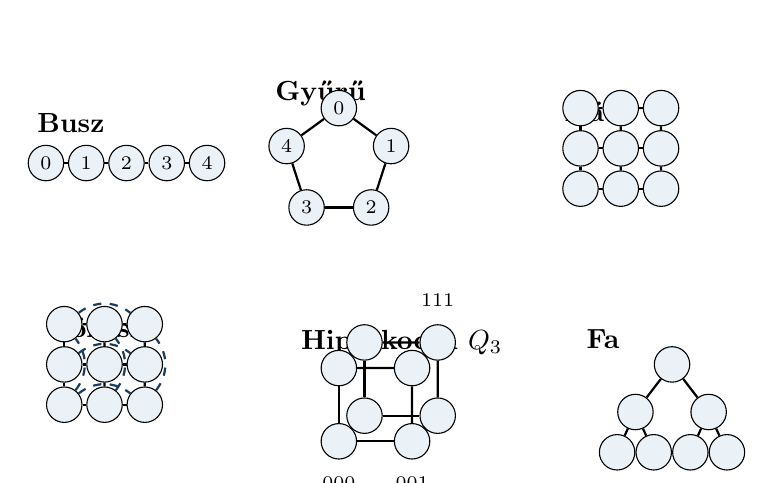
\begin{tikzpicture}[font=\scriptsize, scale=0.93]
  \tikzset{toponode/.style={draw, circle, fill=lightaccent, minimum size=4.5mm, inner sep=0pt},
           topoedge/.style={draw, thick},
           topowrap/.style={draw, thick, dashed, accent!80!black}}

  \begin{scope}[xshift=0cm,yshift=4.7cm]
    \node[anchor=west,font=\bfseries] at (-0.25,0.55) {Busz};
    \foreach \i in {0,...,4} {\node[toponode] (b\i) at (\i*0.55,0) {\i};}
    \foreach \i/\j in {0/1,1/2,2/3,3/4} {\draw[topoedge] (b\i) -- (b\j);}
  \end{scope}

  \begin{scope}[xshift=4.0cm,yshift=4.7cm]
    \node[anchor=west,font=\bfseries] at (-1.0,0.95) {Gyűrű};
    \foreach \i/\a in {0/90,1/18,2/-54,3/-126,4/162} {\node[toponode] (r\i) at (\a:0.75) {\i};}
    \foreach \i/\j in {0/1,1/2,2/3,3/4,4/0} {\draw[topoedge] (r\i) -- (r\j);}
  \end{scope}

  \begin{scope}[xshift=7.3cm,yshift=4.35cm]
    \node[anchor=west,font=\bfseries] at (-0.35,1.05) {Rács};
    \foreach \x in {0,1,2} {\foreach \y in {0,1,2} {\node[toponode] (g\x\y) at (\x*0.55,\y*0.55) {};}}
    \foreach \x in {0,1,2} {\foreach \y/\z in {0/1,1/2} {\draw[topoedge] (g\x\y) -- (g\x\z);}}
    \foreach \y in {0,1,2} {\foreach \x/\z in {0/1,1/2} {\draw[topoedge] (g\x\y) -- (g\z\y);}}
  \end{scope}

  \begin{scope}[xshift=0.25cm,yshift=1.4cm]
    \node[anchor=west,font=\bfseries] at (-0.35,1.05) {Tórusz};
    \foreach \x in {0,1,2} {\foreach \y in {0,1,2} {\node[toponode] (t\x\y) at (\x*0.55,\y*0.55) {};}}
    \foreach \x in {0,1,2} {\foreach \y/\z in {0/1,1/2} {\draw[topoedge] (t\x\y) -- (t\x\z);}}
    \foreach \y in {0,1,2} {\foreach \x/\z in {0/1,1/2} {\draw[topoedge] (t\x\y) -- (t\z\y);}}
    \foreach \x in {0,1,2} {\draw[topowrap] (t\x0) to[bend right=38] (t\x2);}
    \foreach \y in {0,1,2} {\draw[topowrap] (t0\y) to[bend left=38] (t2\y);}
  \end{scope}

  \begin{scope}[xshift=4.0cm,yshift=0.9cm]
    \node[anchor=west,font=\bfseries] at (-0.65,1.35) {Hiperkocka $Q_3$};
    \foreach \x/\y/\n in {0/0/000,1.0/0/001,1.0/1/011,0/1/010,0.35/0.35/100,1.35/0.35/101,1.35/1.35/111,0.35/1.35/110} {
      \node[toponode] (h\n) at (\x,\y) {};
    }
    \foreach \a/\b in {000/001,001/011,011/010,010/000,100/101,101/111,111/110,110/100,000/100,001/101,011/111,010/110} {\draw[topoedge] (h\a) -- (h\b);}
    \node[below=1mm of h000] {000};
    \node[below=1mm of h001] {001};
    \node[above=1mm of h111] {111};
  \end{scope}

  \begin{scope}[xshift=7.8cm,yshift=0.75cm]
    \node[anchor=west,font=\bfseries] at (-0.55,1.55) {Fa};
    \node[toponode] (a) at (0.75,1.2) {};
    \node[toponode] (c) at (0.25,0.55) {};
    \node[toponode] (d) at (1.25,0.55) {};
    \node[toponode] (e) at (0,0) {};
    \node[toponode] (f) at (0.5,0) {};
    \node[toponode] (g) at (1.0,0) {};
    \node[toponode] (i) at (1.5,0) {};
    \foreach \u/\v in {a/c,a/d,c/e,c/f,d/g,d/i} {\draw[topoedge] (\u) -- (\v);}
  \end{scope}
\end{tikzpicture}
\caption{Gyakori kommunikációs topológiák szemléltetése}
\label{fig:zv09_topologiak}
\end{figure}


\section{Busz topológia}

\subsection{Szerkezet}

A busz, más néven lánc topológia olyan gráf, amelyben a csomópontok egy sorba rendezhetők. Jelöljük a csomópontokat $0,1,\ldots,p-1$ indexekkel. Közvetlen él csak a szomszédos csomópontok között van:
\[
  (0,1),(1,2),\ldots,(p-2,p-1).
\]

Az élek száma:
\[
  |E|=p-1.
\]

\subsection{Távolságok}

Két csomópont távolsága a buszon az indexkülönbség abszolútértéke:
\[
  d(i,j)=|i-j|.
\]

A maximális távolság az első és az utolsó csomópont között adódik:
\[
  D=p-1.
\]

A $k$ távolságú, rendezetlen csomópontpárok száma $p-k$, mert $0$ és $k$, $1$ és $k+1$, és így tovább párok választhatók.

Az átlagos távolság rendezetlen csúcspárokra:
\[
  \overline d = \frac{\sum_{k=1}^{p-1} k(p-k)}{\binom{p}{2}} = \frac{p+1}{3}.
\]

\subsection{Értékelés}

Előnye, hogy nagyon egyszerű és kevés összeköttetést igényel. Hátránya, hogy a két végpont között sok közvetítő lépés kellhet, és a középső élek könnyen túlterhelődhetnek.

\section{Gyűrű topológia}

\subsection{Szerkezet}

A gyűrű a busz olyan kiegészítése, ahol az utolsó csomópontot összekötjük az elsővel. Az élek száma:
\[
  |E|=p.
\]

Minden csomópont fokszáma kettő. Az üzenet két irányba indulhat el, ezért a gyűrű a busznál kedvezőbb távolságokat ad.

\subsection{Távolságok}

A $p$ csomópontú gyűrűben két csomópont távolsága:
\[
  d(i,j)=\min(|i-j|,p-|i-j|).
\]

Az átmérő:
\[
  D=\left\lfloor\frac{p}{2}\right\rfloor.
\]

Ha például $p=8$, akkor a legtávolabbi csomópontpárok távolsága $4$, mert a gyűrűn a rövidebb irányt választjuk.

\subsection{Értékelés}

A gyűrű előnye, hogy kevés plusz éllel jelentősen csökkenti a maximális távolságot a buszhoz képest. Hátránya, hogy még mindig viszonylag nagy lehet az átmérő, és hiba esetén a gyűrű megszakadhat, hacsak nincs kerülő út vagy hibakezelés.

\section{Rács topológia}

\subsection{Szerkezet}

A kétdimenziós rácsban a csomópontokat koordinátákkal címezzük:
\[
  (x,y),\qquad 0\leq x<n,
  \quad 0\leq y<m.
\]

A csomópontok száma:
\[
  |V|=nm.
\]

Az élek száma két irányból számolható:
\[
  |E|=(n-1)m+n(m-1)=2nm-n-m.
\]

\subsection{Távolságok}

A rácsban a természetes távolság a Manhattan-távolság:
\[
  d((x_1,y_1),(x_2,y_2))=|x_1-x_2|+|y_1-y_2|.
\]

Az átmérő:
\[
  D=(n-1)+(m-1)=n+m-2.
\]

Például egy $4\times 4$ rácsban a bal alsó és jobb felső sarok távolsága $3+3=6$.

\subsection{Értékelés}

A rács jól illeszkedik olyan feladatokhoz, ahol a bemenet is kétdimenziós vagy lokális szomszédsági kapcsolatokat használ, például képfeldolgozás, numerikus rácsok, szimulációk. Hátránya, hogy a szélső és sarokcsomópontok kevesebb kapcsolattal rendelkeznek, és a távoli sarkok között nagy lehet a távolság.

\section{Tórusz topológia}

\subsection{Szerkezet}

A tórusz a rács olyan változata, amelyben a sorok és oszlopok végeit körbekötjük. Kétdimenziós esetben az $(x,y)$ csomópont szomszédai moduló szerinti koordinátákkal írhatók fel:
\[
  (x\pm 1 \bmod n,y),\qquad (x,y\pm 1 \bmod m).
\]

Ha $n,m>2$, akkor minden csomópont fokszáma $4$, és az élek száma:
\[
  |E|=2nm.
\]

\subsection{Távolságok}

Legyen
\[
  \Delta x=|x_1-x_2|,
  \qquad
  \Delta y=|y_1-y_2|.
\]

A tóruszban a körbekötés miatt minden dimenzióban a rövidebb irányt választjuk:
\[
  d=\min(\Delta x,n-\Delta x)+\min(\Delta y,m-\Delta y).
\]

Az átmérő:
\[
  D=\left\lfloor\frac n2\right\rfloor+
    \left\lfloor\frac m2\right\rfloor.
\]

Egy $4\times 4$ tórusz átmérője $2+2=4$, míg a $4\times 4$ rácsé $6$.

\subsection{Értékelés}

A tórusz előnye, hogy a rácshoz képest csökkenti a maximális és átlagos távolságot, valamint eltünteti a szélek és sarkok hátrányát. Hátránya, hogy több összeköttetést igényel, és a fizikai megvalósítás bonyolultabb lehet.

\section{Hiperkocka topológia}

\subsection{Szerkezet és címzés}

A $d$ dimenziós hiperkocka $Q_d$ csomópontjai $d$ bites bináris címekkel írhatók le. A csomópontok száma:
\[
  |V|=2^d.
\]

Két csomópont akkor szomszédos, ha a bináris címük pontosan egy bitben különbözik. Minden csomópont fokszáma $d$, ezért az élek száma:
\[
  |E|=\frac{2^d\cdot d}{2}=d2^{d-1}.
\]

\subsection{Távolságok}

Két csomópont távolsága a Hamming-távolság, vagyis azoknak a bitpozícióknak a száma, amelyekben a két cím eltér:
\[
  d(u,v)=\operatorname{Hamming}(u,v).
\]

Az átmérő:
\[
  D=d.
\]

Például a $000$ és $111$ című csomópontok távolsága $3$, mert mindhárom bitben eltérnek.

\subsection{Útválasztás}

A hiperkockában egyszerű útválasztási stratégia, hogy minden lépésben kijavítunk egy olyan bitet, amelyben az aktuális cím eltér a célcímtől. Ha $u=0010$ és $v=1111$, akkor három bit különbözik, tehát három lépésben elérhető a cél.

\subsection{Értékelés}

A hiperkocka előnye, hogy a csomópontok száma exponenciálisan nő a dimenzióval, miközben az átmérő csak lineárisan. Jó kommunikációs tulajdonságú topológia, de a dimenzió növekedésével a fokszám is nő, ezért minden csomópontnak egyre több közvetlen kapcsolatra van szüksége.

\section{Fa topológia}

\subsection{Szerkezet}

A fa összefüggő, körmentes gráf. Ha $p$ csomópontja van, akkor az élek száma mindig:
\[
  |E|=p-1.
\]

A csomópontok között pontosan egy egyszerű út vezet. Ez egyszerűvé teszi az útválasztást, de azt is jelenti, hogy bizonyos csomópontok és élek könnyen szűk keresztmetszetté válhatnak.

\subsection{Távolságok}

Két csomópont távolsága a közöttük vezető egyetlen út hossza. Gyökeres fában az út gyakran úgy írható le, hogy az egyik csomóponttól felmegyünk a legkisebb közös őséig, majd lemegyünk a másik csomóponthoz.

Teljes bináris fában, ha a fa magassága $h$, akkor két levél között a maximális távolság legfeljebb:
\[
  D=2h.
\]

\subsection{Értékelés}

A fa hierarchikus rendszerekhez természetes választás. Ilyen például a feladatok rekurzív felosztása, a vezérlő-szolga jellegű kommunikáció vagy bizonyos broadcast és redukciós minták. Hátránya, hogy a gyökér vagy a felső szintű élek túlterhelődhetnek.

\section{Topológiák összehasonlítása}

\begin{center}
{\small
\begin{tabularx}{\textwidth}{L{28mm}L{30mm}X L{25mm}}
\toprule
\textbf{Topológia} & \textbf{Élek száma} & \textbf{Távolság két csúcs között} & \textbf{Átmérő} \\
\midrule
Busz / lánc & $p-1$ & $d(i,j)=|i-j|$ & $p-1$ \\
Gyűrű & $p$ & $d(i,j)=\min(|i-j|,p-|i-j|)$ & $\lfloor p/2\rfloor$ \\
$n\times m$ rács & $(n-1)m+n(m-1)$ & $d=|x_1-x_2|+|y_1-y_2|$ & $(n-1)+(m-1)$ \\
$n\times m$ tórusz & $2nm$ & $d=\min(\Delta x,n-\Delta x)+\min(\Delta y,m-\Delta y)$ & $\lfloor n/2\rfloor+\lfloor m/2\rfloor$ \\
$d$ dimenziós hiperkocka & $d2^{d-1}$ & Hamming-távolság a bináris címek között & $d$ \\
Fa & $p-1$ & Az egyetlen egyszerű út hossza & A leghosszabb csúcspár távolsága \\
\bottomrule
\end{tabularx}
}

\end{center}

Vizsgán érdemes a topológiákat nem csak felsorolni, hanem a következő szempontok alapján összehasonlítani:

\begin{itemize}
  \item mennyi él szükséges;
  \item mennyi a maximális távolság;
  \item mennyire egyszerű a címzés;
  \item mennyire egyszerű az útválasztás;
  \item milyen pontokon alakulhat ki szűk keresztmetszet;
  \item mennyire jól illeszkedik az adott algoritmus kommunikációs mintájához.
\end{itemize}

\begin{warningbox}
Nincs minden helyzetben legjobb topológia. A busz kevés éllel megvalósítható, de nagy lehet az átmérője. A tórusz és a hiperkocka jobb távolságokat adhat, de több összeköttetést és bonyolultabb megvalósítást igényel. A választás mindig a feladat kommunikációs mintájától és a megvalósítás költségétől függ.
\end{warningbox}

\section{CSP modell}

\subsection{Alapgondolat}

A CSP a \textbf{Communicating Sequential Processes} rövidítése. Olyan modell, amelyben a párhuzamosan működő folyamatok nem közös memórián keresztül kommunikálnak, hanem üzeneteket küldenek csatornákon.

A CSP szemléletben:

\begin{itemize}
  \item a folyamatok saját állapottal rendelkeznek;
  \item a kommunikáció csatornákon történik;
  \item az adatátadás explicit művelet;
  \item a közös változók használata helyett az üzenetküldés kerül előtérbe.
\end{itemize}

\subsection{Csatorna}

A csatorna a folyamatok közötti kommunikációs objektum. Egy folyamat adatot küldhet a csatornára, egy másik pedig adatot olvashat róla. A csatorna lehet szinkron vagy pufferelt.

Szinkron csatorna esetén a küldő és a fogadó találkozása szükséges az üzenet átadásához. Pufferelt csatorna esetén a küldő akkor is elhelyezhet üzenetet, ha a fogadó éppen még nem olvassa azt, feltéve hogy a puffer nem telt be.

\subsection{Előnyök és hátrányok}

Előnyök:

\begin{itemize}
  \item csökkenti a közös állapotból adódó versenyhelyzetek esélyét;
  \item a kommunikáció helye a programban jól látható;
  \item természetes módon modellez termelő-fogyasztó és pipeline jellegű feladatokat;
  \item jól illeszkedik olyan nyelvekhez és könyvtárakhoz, amelyek csatornákat biztosítanak.
\end{itemize}

Hátrányok:

\begin{itemize}
  \item rossz csatornahasználat esetén deadlock alakulhat ki;
  \item a kommunikáció sorrendje és blokkoló jellege gondos tervezést igényel;
  \item nagy rendszerekben nehéz lehet áttekinteni, mely folyamat mely csatornán kommunikál.
\end{itemize}

\section{Publish--Subscribe modell}

\subsection{Alapgondolat}

A Publish--Subscribe modellben a kommunikáció nem közvetlen küldő-címzett kapcsolatként jelenik meg. Ehelyett a küldő egy témába, csatornába vagy eseményfolyamba publikál, a feliratkozók pedig megkapják az őket érdeklő témák üzeneteit.

A szereplők:

\begin{itemize}
  \item \textbf{publisher}: üzenetet tesz közzé;
  \item \textbf{topic}: logikai csatorna vagy témakör;
  \item \textbf{subscriber}: feliratkozik egy témára, és értesítést kap;
  \item \textbf{broker}: gyakori megvalósításban közvetítő komponens, amely kezeli a témákat és kézbesítést.
\end{itemize}

\subsection{Működés}

A modell egyszerű vázlata:

\zvpseudocode[caption={Publish--Subscribe működésének vázlata},label={lst:zv09_pubsub_pelda}]{src/code/zv09_pubsub_pelda.pseudo}

A publisher nem feltétlenül tudja, hogy kik a feliratkozók. A subscriber sem feltétlenül ismeri a publisher személyét. Ez laza csatolást eredményez.

\subsection{Előnyök és hátrányok}

Előnyök:

\begin{itemize}
  \item jól skálázható sok fogyasztó esetén;
  \item a küldő és a fogadó lazán kapcsolódik egymáshoz;
  \item eseményvezérelt rendszerekben természetes szervezési mód;
  \item egy üzenet több feliratkozóhoz is eljuthat.
\end{itemize}

Hátrányok:

\begin{itemize}
  \item nehezebb lehet követni, hogy egy üzenet pontosan hová jut el;
  \item a kézbesítési garanciák megvalósítástól függnek;
  \item ha központi broker van, az szűk keresztmetszet vagy hibapont lehet;
  \item a hibakezelés és újrapróbálás összetettebb lehet.
\end{itemize}

\section{Aktor modell}

\subsection{Alapgondolat}

Az Aktor modellben az alapegység az \textbf{aktor}. Az aktor önálló, izolált állapottal rendelkező entitás, amely üzeneteket fogad és dolgoz fel. Kívülről az állapota közvetlenül nem módosítható.

Egy aktor üzenet feldolgozásakor tipikusan a következőket teheti:

\begin{enumerate}
  \item módosíthatja saját belső állapotát;
  \item üzenetet küldhet más aktoroknak;
  \item új aktort hozhat létre;
  \item meghatározhatja, hogyan viselkedjen a következő üzeneteknél.
\end{enumerate}

\subsection{Cím, postaláda és üzenet}

Az aktoroknak címük van, amelyre üzenetet lehet küldeni. Minden aktorhoz tartozik egy postaláda, vagyis üzenetsor. Az aktor ebből veszi ki a feldolgozandó üzeneteket. A modellben gyakori feltételezés, hogy egy aktor egyszerre egy üzenetet dolgoz fel, ezért a saját állapotát nem kell több szál ellen védenie.

Az elküldött üzeneteket célszerű változtathatatlan adatként kezelni, mert így elkerülhető, hogy két aktor ugyanazt az objektumot egyszerre módosítsa.

\begin{figure}[htbp]
\centering
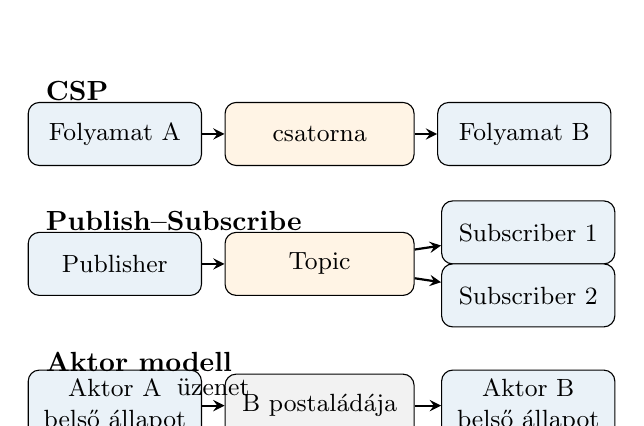
\begin{tikzpicture}[font=\small, node distance=8mm]
  \tikzset{proc/.style={draw, rounded corners, fill=lightaccent, minimum width=22mm, minimum height=8mm, align=center},
           chan/.style={draw, rounded corners, fill=warnbg, minimum width=24mm, minimum height=8mm, align=center},
           mailbox/.style={draw, rounded corners, fill=black!5, minimum width=24mm, minimum height=8mm, align=center},
           msg/.style={->, >=stealth, thick}}

  \node[proc] (cspA) at (0,2.2) {Folyamat A};
  \node[chan] (cspC) at (2.6,2.2) {csatorna};
  \node[proc] (cspB) at (5.2,2.2) {Folyamat B};
  \draw[msg] (cspA) -- (cspC);
  \draw[msg] (cspC) -- (cspB);
  \node[anchor=west,font=\bfseries] at (-1.0,2.75) {CSP};

  \node[proc] (pub) at (0,0.55) {Publisher};
  \node[chan] (topic) at (2.6,0.55) {Topic};
  \node[proc] (sub1) at (5.25,0.95) {Subscriber 1};
  \node[proc] (sub2) at (5.25,0.15) {Subscriber 2};
  \draw[msg] (pub) -- (topic);
  \draw[msg] (topic) -- (sub1);
  \draw[msg] (topic) -- (sub2);
  \node[anchor=west,font=\bfseries] at (-1.0,1.1) {Publish--Subscribe};

  \node[proc] (act1) at (0,-1.25) {Aktor A\\belső állapot};
  \node[mailbox] (mail) at (2.6,-1.25) {B postaládája};
  \node[proc] (act2) at (5.25,-1.25) {Aktor B\\belső állapot};
  \draw[msg] (act1) -- node[above] {üzenet} (mail);
  \draw[msg] (mail) -- (act2);
  \node[anchor=west,font=\bfseries] at (-1.0,-0.7) {Aktor modell};
\end{tikzpicture}
\caption{Üzenetküldési modellek kapcsolati szerkezete}
\label{fig:zv09_uzenetkuldesi_modellek}
\end{figure}


\subsection{Supervision}

Az Aktor modell gyakorlati megvalósításaiban gyakori a felügyeleti fa. Egy aktor felügyelheti a gyermekaktorokat, és hiba esetén újraindíthatja vagy leállíthatja őket. Ez hibatűrő rendszerekben előnyös, mert a hibakezelés szervezetten épül be a modellbe.

\subsection{Előnyök és hátrányok}

Előnyök:

\begin{itemize}
  \item jól elkülöníti az állapotokat;
  \item csökkenti a közös memória miatti versenyhelyzeteket;
  \item jól skálázható sok független egységre;
  \item hibatűrő rendszerekben jól használható a supervision szemlélet miatt.
\end{itemize}

Hátrányok:

\begin{itemize}
  \item az üzenetsorrend és kézbesítés részletei megvalósítástól függhetnek;
  \item a postaládák túlcsordulhatnak;
  \item a hibák aszinkron módon jelenhetnek meg, ezért nehezebb lehet nyomkövetni őket;
  \item deadlock vagy livelock logikai szinten továbbra is kialakulhat.
\end{itemize}

\section{CSP, Publish--Subscribe és Aktor modell összehasonlítása}

\begin{center}
\begin{tabularx}{\textwidth}{L{28mm}L{31mm}L{35mm}X}
\toprule
\textbf{Modell} & \textbf{Kapcsolat} & \textbf{Állapotkezelés} & \textbf{Fő gondolat} \\
\midrule
CSP & Folyamatok csatornákon keresztül & Nincs közös memória; a folyamatok saját állapottal dolgoznak & A kommunikációt csatornák szervezik. A folyamatok nem közös változókat írnak, hanem üzeneteket adnak át. \\
Publish--Subscribe & Kiadók, témák és feliratkozók & A kiadó és a feliratkozó laza kapcsolatban van; gyakran közvetítő kezeli a témákat & A kiadó egy témába publikál, a feliratkozók pedig megkapják az adott témához tartozó üzeneteket. \\
Aktor modell & Aktorok egymás címeire küldenek üzenetet & Minden aktor saját, kívülről nem módosítható belső állapottal és postaládával rendelkezik & Az aktor üzenetet fogad, állapotot módosíthat, új üzenetet küldhet és új aktort hozhat létre. \\
\bottomrule
\end{tabularx}

\end{center}

A három modell közös célja, hogy a párhuzamos és elosztott komponensek kommunikációját kezelhetőbbé tegye. A különbség főleg abban van, hogy ki tud kiről, és mi a kommunikáció központi fogalma.

\begin{itemize}
  \item CSP-ben a csatorna a központi elem. A folyamatok csatornákon keresztül kommunikálnak.
  \item Publish--Subscribe esetén a téma vagy eseménycsatorna a központi elem. A kiadó és a feliratkozó laza kapcsolatban van.
  \item Aktor modellben az aktor címe és postaládája a központi elem. Az aktorok egymásnak küldenek üzenetet.
\end{itemize}

Vizsgán hasznos megfogalmazás: CSP-ben a folyamatok csatornákon beszélnek, Publish--Subscribe modellben a szereplők témákon keresztül értesülnek eseményekről, az Aktor modellben pedig önálló állapotú aktorok küldenek egymás postaládájába üzeneteket.

\section{Aszinkron programozás}

\subsection{Konkurrencia és párhuzamosság}

Az aszinkron programozás megértéséhez először külön kell választani a konkurrenciát és a párhuzamosságot.

\textbf{Konkurrencia} esetén több tevékenységet szervezünk úgy, hogy időben átfedésben haladhassanak. Ez akkor is lehetséges, ha fizikailag csak egy végrehajtó szál van, mert a program várakozási pontokon átadhatja a vezérlést.

\textbf{Párhuzamosság} esetén több tevékenység ténylegesen ugyanabban az időpillanatban fut, például több CPU-magon.

Az aszinkron programozás fő célja gyakran nem a CPU-intenzív számítások gyorsítása, hanem az, hogy a program ne blokkoljon feleslegesen I/O-műveletek, hálózati kérések, fájlműveletek vagy időzítők miatt.

\subsection{Event loop szemlélet}

Az aszinkron futtatókörnyezetben gyakran van egy \textbf{event loop}. Ez figyeli, hogy mely műveletek készültek el, és mikor lehet folytatni a hozzájuk tartozó feladatot.

Egy leegyszerűsített működés:

\begin{enumerate}
  \item egy aszinkron művelet elindul;
  \item a program nem vár blokkoló módon, hanem visszaadja a vezérlést az event loopnak;
  \item amikor az eredmény elkészül, az event loop folytatja a megfelelő coroutine-t;
  \item a folytatás az \code{await} utáni ponttól történik.
\end{enumerate}

\subsection{Async és await}

Az \code{async} kulcsszó általában azt jelzi, hogy egy függvény aszinkron módon futtatható. A függvény meghívása sok nyelvben nem közvetlenül a végeredményt adja vissza, hanem egy olyan objektumot, amely a későbbi eredményt képviseli. Ez lehet például Promise, Future, Task vagy coroutine objektum.

Az \code{await} kulcsszó azt jelenti, hogy az aktuális aszinkron végrehajtási egység megvárja egy aszinkron művelet eredményét, de közben nem feltétlenül blokkolja az egész programot vagy az event loopot.

\begin{warningbox}
Az \code{await} nem ugyanaz, mint egy egyszerű blokkoló várakozás. Jó aszinkron futtatókörnyezetben az \code{await} felfüggeszti az aktuális coroutine-t, és lehetőséget ad más feladatok futtatására. Ha viszont az aszinkron függvényen belül blokkoló műveletet hívunk, akkor az egész event loop is megakadhat.
\end{warningbox}

\section{Coroutine-ok}

\subsection{Fogalom}

A coroutine olyan végrehajtási egység, amely felfüggeszthető és később ugyanonnan folytatható. A hagyományos függvényhívás belép a függvénybe, majd a függvény visszatér. A coroutine ezzel szemben több részletben is futhat: bizonyos pontokon átadja a vezérlést, majd később folytatódik.

A coroutine-ok gyakran kooperatív multitaskingot valósítanak meg. Ez azt jelenti, hogy a váltás nem tetszőleges gépi utasításnál történik, hanem jól meghatározott felfüggesztési pontokon, például \code{await} kifejezéseknél.

\subsection{Miért hasznos?}

Coroutine-ok segítségével sok olyan feladat kezelhető hatékonyan, amely sokat vár külső eseményre:

\begin{itemize}
  \item hálózati kérés válaszára;
  \item fájlművelet befejezésére;
  \item adatbázis-lekérdezésre;
  \item időzítő lejárására;
  \item felhasználói eseményre.
\end{itemize}

Ilyenkor a várakozó feladat felfüggeszthető, és a futtatókörnyezet más feladatokat végezhet.

\section{Aszinkron példák}

\subsection{JavaScript példa}

A következő példa két aszinkron munkát indít. A munkák nem egymás után várakoznak le, hanem egyszerre elindulnak, majd a \code{Promise.all} várja meg mindkettő befejezését.

\zvcode[caption={Egyszerű JavaScript async/await példa},label={lst:zv09_async_js}]{src/code/zv09_async_js.js}

Fontos részlet, hogy a \code{worker("A", 2000)} és a \code{worker("B", 1000)} hívás eredményét először eltároljuk. Így a két várakozás időben átfedésbe kerülhet. Ha ehelyett az első hívást rögtön \code{await}-elnénk, akkor a második csak később indulna el.

\subsection{Python példa}

Pythonban az \code{async def} coroutine függvényt hoz létre. A \code{create\_task} elindítja az ütemezhető feladatot, az \code{asyncio.gather} pedig több feladat befejezését várja meg.

\zvcode[caption={Egyszerű Python asyncio coroutine példa},label={lst:zv09_async_python}]{src/code/zv09_async_python.py}

A példában az \code{asyncio.sleep} nem blokkoló várakozás. Ez azért lényeges, mert a coroutine ilyenkor átadja a vezérlést az event loopnak, és más coroutine folytatódhat.

\section{Aszinkron fogalmak összefoglalása}

\begin{center}
\begin{tabularx}{\textwidth}{L{31mm}X}
\toprule
\textbf{Fogalom} & \textbf{Jelentés} \\
\midrule
Konkurrencia & Több tevékenység végrehajtása időben átfedésben szervezhető. Nem feltétlenül jelent több processzormagon futó valódi párhuzamosságot. \\
Párhuzamosság & Több tevékenység ténylegesen ugyanabban az időben fut, például több processzormagon. \\
Aszinkron végrehajtás & A program nem blokkol minden várakozásnál, hanem a futtatókörnyezet más feladatot is futtathat. \\
Coroutine & Olyan végrehajtási egység, amely bizonyos pontokon felfüggeszthető, majd később ugyanonnan folytatható. \\
\code{async} & Aszinkron függvény vagy coroutine létrehozását jelzi. Sok nyelvben a visszatérési érték ígéret, task vagy coroutine objektum. \\
\code{await} & Felfüggeszti az aktuális aszinkron végrehajtási egységet addig, amíg a várt művelet eredménye elkészül. \\
Event loop & Olyan ütemező ciklus, amely figyeli az elkészült aszinkron műveleteket, és folytatja a hozzájuk tartozó coroutine-okat. \\
Promise / Future / Task & Egy később elkészülő eredmény objektumszerű reprezentációja. Lehet sikeres, hibás vagy még folyamatban lévő állapotban. \\
\bottomrule
\end{tabularx}

\end{center}

\section{Gyakori félreértések}

\subsection{Az async nem feltétlenül jelent több processzormagot}

Az \code{async}/\code{await} használata önmagában nem garantál valódi párhuzamos végrehajtást. Sok futtatókörnyezetben az aszinkron kód egyetlen szálon, event loop segítségével szerveződik. Ez I/O-várakozásnál nagyon hatékony lehet, de CPU-intenzív feladatnál nem feltétlenül gyorsít.

CPU-intenzív számításhoz gyakran külön szálakra, folyamatokra, párhuzamos könyvtárakra, GPU-ra vagy más valódi párhuzamosítási megoldásra van szükség.

\subsection{Az await helye számít}

Ha egy aszinkron műveletet rögtön \code{await}-elünk, akkor a következő művelet csak az előző befejezése után indulhat. Ha több független művelet van, akkor előbb célszerű őket elindítani, és utána közösen megvárni az eredményt.

\subsection{Az üzenetküldés nem szüntet meg minden hibát}

A CSP, Publish--Subscribe és Aktor modell csökkenti a közös állapotból adódó hibák egy részét, de nem teszi automatikusan hibamentessé a rendszert. Továbbra is figyelni kell a holtpontokra, túlcsorduló sorokra, elveszett üzenetekre, sorrendi problémákra és hibakezelésre.

\section{Tipikus vizsgakérdések és rövid válaszvázlatok}

\subsection{Mit jelent egy topológia átmérője?}

Az átmérő a legnagyobb legrövidebb úthossz két csomópont között. Kommunikációs szempontból azt mutatja meg, hogy legrosszabb esetben hány lépés kell két csomópont közötti üzenetküldéshez.

\subsection{Mi a busz és a gyűrű fő különbsége?}

A busz láncszerű, $p-1$ élű topológia, átmérője $p-1$. A gyűrű a buszt kiegészíti az utolsó és az első csomópont közötti éllel, ezért $p$ éle van, átmérője pedig $\lfloor p/2\rfloor$.

\subsection{Hogyan számítjuk a rács és a tórusz távolságát?}

Rácsban Manhattan-távolságot használunk. Tóruszban minden dimenzióban a körbekötés miatt a rövidebb irányt választjuk, ezért a távolság dimenziónként $\min(\Delta,n-\Delta)$ alakú.

\subsection{Miért előnyös a hiperkocka?}

A $d$ dimenziós hiperkockában $2^d$ csomópont van, de az átmérő csak $d$. A távolság a bináris címek Hamming-távolsága, ezért az útválasztás egyszerűen végezhető bitenként.

\subsection{Mi a CSP lényege?}

A CSP-ben párhuzamos folyamatok kommunikálnak csatornákon keresztül. A modell nem a közös memória módosítását helyezi előtérbe, hanem az explicit üzenetátadást.

\subsection{Mi a Publish--Subscribe modell előnye?}

Laza csatolást ad a kiadó és a feliratkozók között. A kiadó egy témába publikál, a feliratkozók pedig a témára feliratkozva kapják meg az üzeneteket. Így egy üzenet több fogyasztóhoz is eljuthat.

\subsection{Mi az Aktor modell alapegysége?}

Az aktor. Minden aktor saját állapottal és postaládával rendelkezik. Üzenetet fogad, saját állapotot módosíthat, üzenetet küldhet, és új aktort hozhat létre.

\subsection{Mire való az async és az await?}

Az \code{async} aszinkron függvényt vagy coroutine-t jelöl, az \code{await} pedig egy aszinkron művelet eredményére vár úgy, hogy közben az aktuális coroutine felfüggeszthető, és a futtatókörnyezet más feladatokat futtathat.

\section{Összefoglalás vizsgára}

Rövid, vizsgán jól használható összefoglalás:

\begin{itemize}
  \item A kommunikációs topológia gráfként modellezhető: a csomópontok számítási egységek, az élek kommunikációs kapcsolatok.
  \item A távolság a legrövidebb út hossza, az átmérő pedig a legnagyobb csomóponttávolság.
  \item Buszban $d(i,j)=|i-j|$, $|E|=p-1$, az átmérő $p-1$.
  \item Gyűrűben $d(i,j)=\min(|i-j|,p-|i-j|)$, $|E|=p$, az átmérő $\lfloor p/2\rfloor$.
  \item Rácsban Manhattan-távolságot használunk, az $n\times m$ rács átmérője $n+m-2$.
  \item Tóruszban a rács szélei körbe vannak kötve, ezért az átmérő $\lfloor n/2\rfloor+\lfloor m/2\rfloor$.
  \item Hiperkockában a csomópontok bináris címek, a távolság Hamming-távolság, az átmérő $d$.
  \item Fában két csomópont között egyetlen egyszerű út van, ezért az útválasztás egyszerű, de felső szinteken szűk keresztmetszet alakulhat ki.
  \item CSP-ben a folyamatok csatornákon kommunikálnak, közös memória helyett üzenetátadással.
  \item Publish--Subscribe modellben a publisher témába publikál, a subscriberek pedig a témára feliratkozva kapnak üzenetet.
  \item Aktor modellben az aktorok izolált állapottal és postaládával rendelkeznek, és egymásnak üzeneteket küldenek.
  \item Az \code{async}/\code{await} a várakozó műveletek nem blokkoló kezelését segíti. Ez főleg I/O-intenzív feladatoknál hasznos.
  \item A coroutine felfüggeszthető és később folytatható végrehajtási egység, amelyet gyakran event loop ütemez.
\end{itemize}

\end{document}
